\section{Explaining Type Errors With Traces}
\label{sec:explaining}
%
We have shown how to reliably find witnesses to type errors in \ocaml,
but this not fully address our original goal -- to \emph{explain} the
errors.
%
Having identified an input vector that triggers a bug, a common next
step is to step through the program with a \emph{debugger} to observe
how the program evolves.
%
The existing debuggers and interpreters for \ocaml assume a type-correct
program, so unfortunately we cannot use them off-the-shelf.
%
Instead we return to our semantics for \lang and extend the evaluation
rules to collect a trace that we can present to the user, demonstrating
precisely \emph{how} their program went wrong.

The trace takes the form of a \emph{reduction graph}, where the nodes
are terms and the edges represent either the single-step
$\hookrightarrow$ or a ``sub-term'' relation. For example, evaluating
the expression @1 + 2 + 3@ would produce the graph in
Figure~\ref{fig:simple-reduction}.
%
\begin{figure}[t]
  \centering
  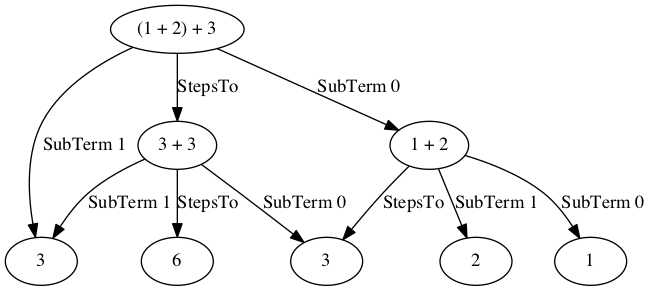
\includegraphics[width=\linewidth]{simple.png}
\caption{The reduction graph for \texttt{1 + 2 + 3}.}
\label{fig:simple-reduction}
\end{figure}
%
We choose this graph representation instead of a simple, linear sequence
of expressions because it will allow us to express a variety of
traversals, such as ``step into'' and ``step over'' -- commonly found in
traditional debuggers.

\subsection{Interactive Semantics}
\label{sec:inter-semant}
%
\begin{figure*}[t]
\relDescription{Trace Syntax}
$$
\begin{array}{rrcl}
  & \tr & ::= & \bullet \spmid \singlestep{e}{e}; \tr \spmid \subterm{e}{e}; \tr
\end{array}
$$
\\
\relDescription{\subtermssym}
\begin{gather*}
\begin{array}{lcl}
\subterms{\eapp{e_1}{e_2}}   & \defeq & \subterm{\eapp{e_1}{e_2}}{e_1}; \subterm{\eapp{e_1}{e_2}}{e_2} \\
\subterms{\eplus{e_1}{e_2}}   & \defeq & \subterm{\eplus{e_1}{e_2}}{e_1}; \subterm{\eplus{e_1}{e_2}}{e_2} \\
\subterms{\eif{e_1}{e_2}{e_3}}   & \defeq & \subterm{\eif{e_1}{e_2}{e_3}}{e_1}; \\
                                &        & \subterm{\eif{e_1}{e_2}{e_3}}{e_2}; \\ 
                                &        & \subterm{\eif{e_1}{e_2}{e_3}}{e_3} \\
\subterms{\elet{x}{e_1}{e_2}}   & \defeq & \subterm{\elet{x}{e_1}{e_2}}{e_1}; \\
                                &        & \subterm{\elet{x}{e_1}{e_2}}{e_2} \\
\subterms{\efun{x}{e}}       & \defeq & \subterm{\efun{x}{e}}{e} \\
\subterms{e}                 & \defeq & \bullet
\end{array}
\end{gather*}
\judgementHead{Evaluation}{\stepg{e}{\su}{\tr}{e}{\su}{\tr}}
\begin{gather*}
\inference[\recontext]
  {\stepg{e}{\su}{\tr}{e_1}{\su_1}{\tr_1}}
  {\stepg{C[e]}{\su}{\tr}{C[e_1]}{\su_1}{\singlestep{C[e]}{C[e_1]}; \subterms{C[e_1]}; \tr_1}} 
\\ \\
\inference[\reappgood]
  {\pair{\efun{x}{e}}{\su_2} = \force{v_1}{\tfun{\thole{}}{\thole{}}}}
  {\stepg{\eapp{v_1}{v_2}}{\su_1}{\tr}
         {e\sub{x}{v_2}}{\su_1\su_2}{\singlestep{\eapp{v_1}{v_2}}{e\sub{x}{v_2}}; \subterms{e\sub{x}{v_2}}; \tr}}
\\ \\
\inference[\reappbad]
  {\pair{\stuck}{\su_2} = \force{v_1}{\tfun{\thole{}}{\thole{}}}}
  {\stepg{\eapp{v_1}{v_2}}{\su_1}{\tr}{\stuck}{\su_1\su_2}{\singlestep{\eapp{v_1}{v_2}}{\stuck}; \tr}}
\end{gather*}
\caption{A selection of the operational semantics from
  Figure~\ref{fig:operational}, extended to collect a full reduction
  graph.}
\label{fig:interactive}
\end{figure*}
%
The changes to the operational semantics of \S\ref{sec:semantics} are
mechanical, so we will not reproduce them in full; instead we describe
the procedure for extending a transition rule and provide a selection of
examples in Figure~\ref{fig:interactive}.

First, we extend the transition relation to collect a set of edges from
which we will construct the graph. 
%
An edge between two expressions is either a ``steps-to'' edge -- written
\singlestep{e_1}{e_2} -- indicating that $e_1$ transitions to $e_2$ in a
single step, or a ``sub-term'' edge -- written \subterm{e_1}{e_2} --
indicating that $e_1$ contains $e_2$ as a sub-expression.
%
Collecting the steps-to edges is a simple matter of recording the
consequent of each original rule in the trace; each original judgment
\step{e_1}{\su_1}{e_2}{\su_2} becomes 
\stepg{e_1}{\su_1}{\tr_1}{e_2}{\su_2}{\singlestep{e_1}{e_2}; \tr_1}.
%
The sub-term edges can be delegated to a new \subtermssym helper
function, which adds edges from an expression to each of its
\emph{immediate} sub-expressions.
%
We collect new sub-term edges after each transition, thus the final
template for the small-step relation is:
$$
\stepg{e_1}{\su_1}{\tr_1}{e_2}{\su_2}{\singlestep{e_1}{e_2}; \subterms{e_2}; \tr_1}
$$



% \begin{itemize}
% \item extend operational semantics to collect reduction graph
% \item nodes are terms, edges indicate ``steps-to'' and ``sub-term'' relations
% \item visualize path through reduction graph
% \item expand edges to reveal more fine-grained steps (step/jump forward/backward)
% \item never lose context (unlike traditional debugger)
% \end{itemize}
